\icode[purple]{E-MM-MU-L4-260625-004}
（多选）
如图所示，半径为\(R\)的光滑半球放在光滑水平面上，将一小滑块（可视为质点）轻放在半球的顶端，小滑块和半球均处于静止状态。在外界微小扰动下，小滑块从静止开始沿球面自由滑下，当小滑块与球心连线与竖直方向夹角\(\theta =\) \,\qty{37}{\degree}时，小滑块离开球面。重力加速度为\(g\)，\(\sin\) \,\qty{37}{\degree}\( = 0.6\)，\(\cos\) \,\qty{37}{\degree}\( = 0.8\)，下列说法正确的是\paren[]

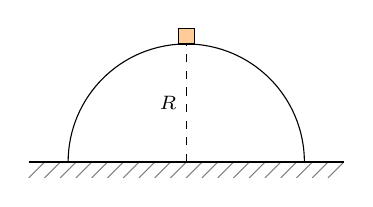
\begin{tikzpicture}
    \draw (1.5,0) arc(0:180:1.5);
    \foreach \x in{-2,-1.8,...,1.8}
        \draw[gray] (\x,-.2)--++(.2,.2);
    \draw[thick] (-2,0)--(2,0);
    \draw[dashed] (0,0)--node[left,font=\scriptsize]{\(R\)}(0,1.5);
    \draw[fill=orange!40] (-.1,1.5) rectangle(.1,1.7);
\end{tikzpicture}
\begin{choices}
    \item 小滑块在球面上滑动过程中，小滑块与半球组成的系统动量守恒
    \item 小滑块在球面上滑动过程中，小滑块与半球组成的系统机械能守恒
    \item 小滑块离开半球时，半球的速度大小为\(\frac{\sqrt{5gR}}{4}\)
    \item 小滑块离开半球时，半球移动的距离为\(\frac{17}{32}R\)
\end{choices}
\begin{answer}
    BC\quad 提示：

    \begin{tikzpicture}[font=\scriptsize,>=latex]
        \draw[gray] (2,0) arc(0:180:2);
        \foreach \x in{-2.4,-2.2,...,2.2}
            \draw[gray] (\x,-.2)--++(.2,.2);
        \draw[thick] (-2.4,0)--(2.4,0);
        \draw[dashed] (0,0)--(53:2)coordinate(a);
        \draw[->,red] (a)--++(-37:1.6)coordinate(u)node[right]{\(u\)};
        \draw[->,blue] (a)--++(0:-1)coordinate(c)node[left]{\(v_2\)};
        \draw[->,cyan] (a)--++($(-37:1.6)+(-1,0)$)coordinate(b)node[below]{\(v_1\)};
        \draw[dashed] (c)--(b)--(u)|-(a) (b)|-(a-|2,1.6);
        \draw[->,cyan] (a)--++(.3,0)node[above]{\(v_{1x}\)};
        \fill (a) circle(.03) (0,0) circle(.03);
    \end{tikzpicture}

    小滑块的速度\(v_1\)、半球的速度\(v_2\)及滑块相对半球的速度\(u\)的关系如图所示，小滑块质量\(m\)、半球质量\(M\)系统水平方向动量守恒：\( Mv_2 =mv_{1x} = m(u\cos\theta - v_2)\)

    由能量守恒可得：\(mgR(1 -\cos\theta) = \frac{1}{2}Mv_2^2 + \frac{1}{2}mv_1^2 = \frac{1}{2}Mv_2^2 + \frac{1}{2}m[(u\sin\theta)^2 +(u\cos\theta - v_2)^2]\)

    小滑块相对半球做圆周运动，\(\theta =\) \,\qty{37}{\degree}时恰好脱离，可得：\(mg\cos\theta = m \frac{u^2}{R}\)

    解得：\(M:m = 7:25\)\quad \(u = \frac{2 \sqrt{5gR}}{5}\)\quad \(v_2 = \frac{\sqrt{5gR}}{4}\)\quad \(x_2 = \frac{25}{7 + 25}\cdot R\sin\theta = \frac{15}{32}R\)
\end{answer}